\documentclass[aps,pra,notitlepage,amsmath,amssymb,letterpaper,12pt]{revtex4-1}
\usepackage{amsthm}
\usepackage{graphicx}
%  Above uses the Americal Physical Society template for Physical Review A
%  as a reasonable and fully-featured default template
 
%  Below define helpful commands to set up problem environments easily
\newenvironment{problem}[2][Problem]{\begin{trivlist}
\item[\hskip \labelsep {\bfseries #1}\hskip \labelsep {\bfseries #2.}]}{\end{trivlist}}
\newenvironment{solution}{\begin{proof}[Solution]}{\end{proof}}
 
% --------------------------------------------------------------
%                   Document Begins Here
% --------------------------------------------------------------
 
\begin{document}
 
\title{CS510 CW 1}
\author{Evan Walker and Ehsan Yaghmaei}
\affiliation{CS 510, Schmid College of Science and Technology, Chapman University}
\date{\today}

\maketitle

\section{Derivative Definition} % Specify main sections this way
% 1 is the problem number

How to define a derivative of a function.

 
\textbf{Definition}  %You can also use proof in place of solution
The derivative of  $f(x)$ with respect to x is the function $f'(x)$ and is defined as,
\begin{align}
f'(x) &= \lim_{h \to 0}\frac{f(x + h) - f(x)}{h}
\end{align}

\subsection{Find a Derivative} % Specify subsections and subsubsections this way

To find the derivative of a function y = f(x) we use the slope formula:

\begin{align}
$Slope $ = \frac{Change\hspace{.1cm}in\hspace{.1cm}Y}{Change\hspace{.1cm}in \hspace{.1cm}X} &= \frac{\Delta x}{\Delta y} 
\end{align}


Above\\
X changes from x to (x+$\Delta$x)\\
Y changes from f(x) to f(x + $\Delta$x)\\
\\
Then\\
Fill in this slope formula:\\
\begin{align}
\frac{\Delta y}{\Delta x} &= \frac{f(x +\Delta x) - f(x)}{\Delta x} 
\end{align}

Simplify the expression as much as we can,\\
Then let $\Delta$x approach zero.\\
\begin{problem}{1}
Let $f(x) = x^2$ and calculate f(x +\Delta x)\\

Start with:\\
\begin{align}
f(x +\Delta x) = (x +\Delta x)^2
\end{align}

Expand:\\
\begin{align}
f(x +\Delta x) = x^2 + 2x\Delta x +(\Delta x)^2
\end{align}
Plug the expanded into the slope formula:

\begin{align}
\frac{x^2 + 2x\Delta x +(\Delta x)^2 - x^2}{\Delta x} 
\end{align}

Here $x^2$ and $-x^2$ cancel and the numerator divide through by \Delta x.

Result:
\begin{align}
f'(x) &= 2x
\end{align}

\subsection{Who discovered derivative ?} % Specify subsections and subsubsections this way

Calculus, known in its early history as infinitesimal calculus, is a mathematical discipline focused on limits, functions, derivatives, integrals, and infinite series. Isaac Newton discovered calculus in the mid-17th century(simultaneously with GottFried Leibniz).

\begin{figure}[h!] % h forces the figure to be placed here, in the text
  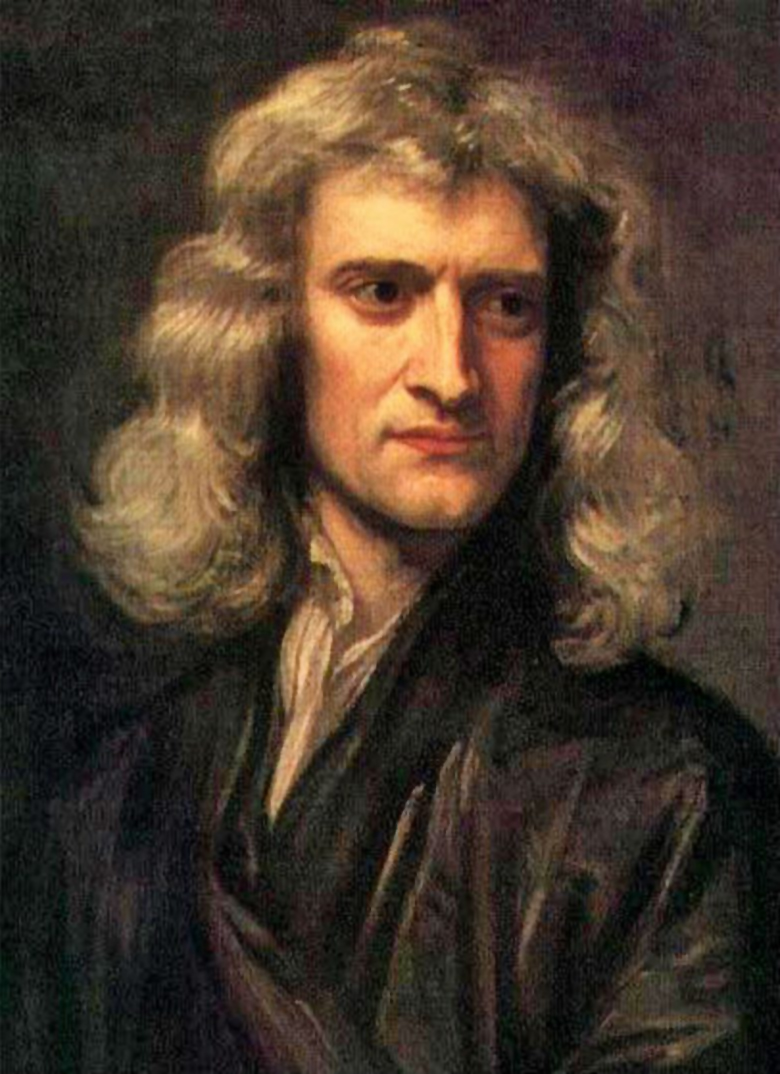
\includegraphics[width=0.4\textwidth]
  {GodfreyKneller-IsaacNewton-1689.jpg}  % if pdflatex is used, jpg, pdf, and png are permitted
  \caption{Around the 1670s, Sir Isaac Newton's conceptual understanding of physics prompted him to invent the complicated math known as calculus.}
  \label{fig:figlabel}
\end{figure}

\end{problem}

\end{document}